\documentclass{bhcguides}

\usepackage[legalpaper, portrait, margin=1.2in]{geometry}
\usepackage[utf8]{inputenc}
\usepackage{tabu}
\setlength{\parindent}{0pt}
\setlength{\parskip}{6 pt}

\usepackage{graphicx}
\graphicspath{ {images/} }

\usepackage{url}
\usepackage{hyperref}
\usepackage{cite}

\begin{document}

\title{Service User Manual}

\includegraphics[width=1.0\textwidth]{BHCbanner.png}
\date{\today}
\maketitle

\tableofcontents

\section{Overview}

The Building Healthy Communities programme is a partnership that delivers a range of initiatives, activites, interventions and skills classes to improve the wellbeing of the community as a whole, and the members of that community. That includes you, the service user. But if you've come this far, you already know that. What you want to know is, what's this website got to do with anything, and how do I use it? That's where this manual comes in.

The Building Healthy Communities website is a fast, convenient way for you to access details about the initiatives you are enrolled in, times for the next meetings, and details the system holds about you, alongside being a quick and easy way to leave feedback for those running the initiatives. The website also features contact details and a way to request changes to your own details, contact or otherwise. This manual will walk you through the process of logging in, viewing your details and initiatives, and leaving feedback. It will also give additional guides on how to contact staff members, and what to do if you lose your login details.

\pagebreak

\section{System Access and Login}
\label{sec:syslogin}

The website is currently hosted at \url{http://hidden-mountain-49766.herokuapp.com} , which can be accessed through most major web browsers (Chrome, Firefox, Safari, IE8 or higher). Before accessing the site, you should have your email address and password (given to you by an administrator) on hand. Upon entering the website, you will be taken to the login page, as seen in \autoref{fig:initialLogin}.

\begin{figure}[h!]
 \centerline{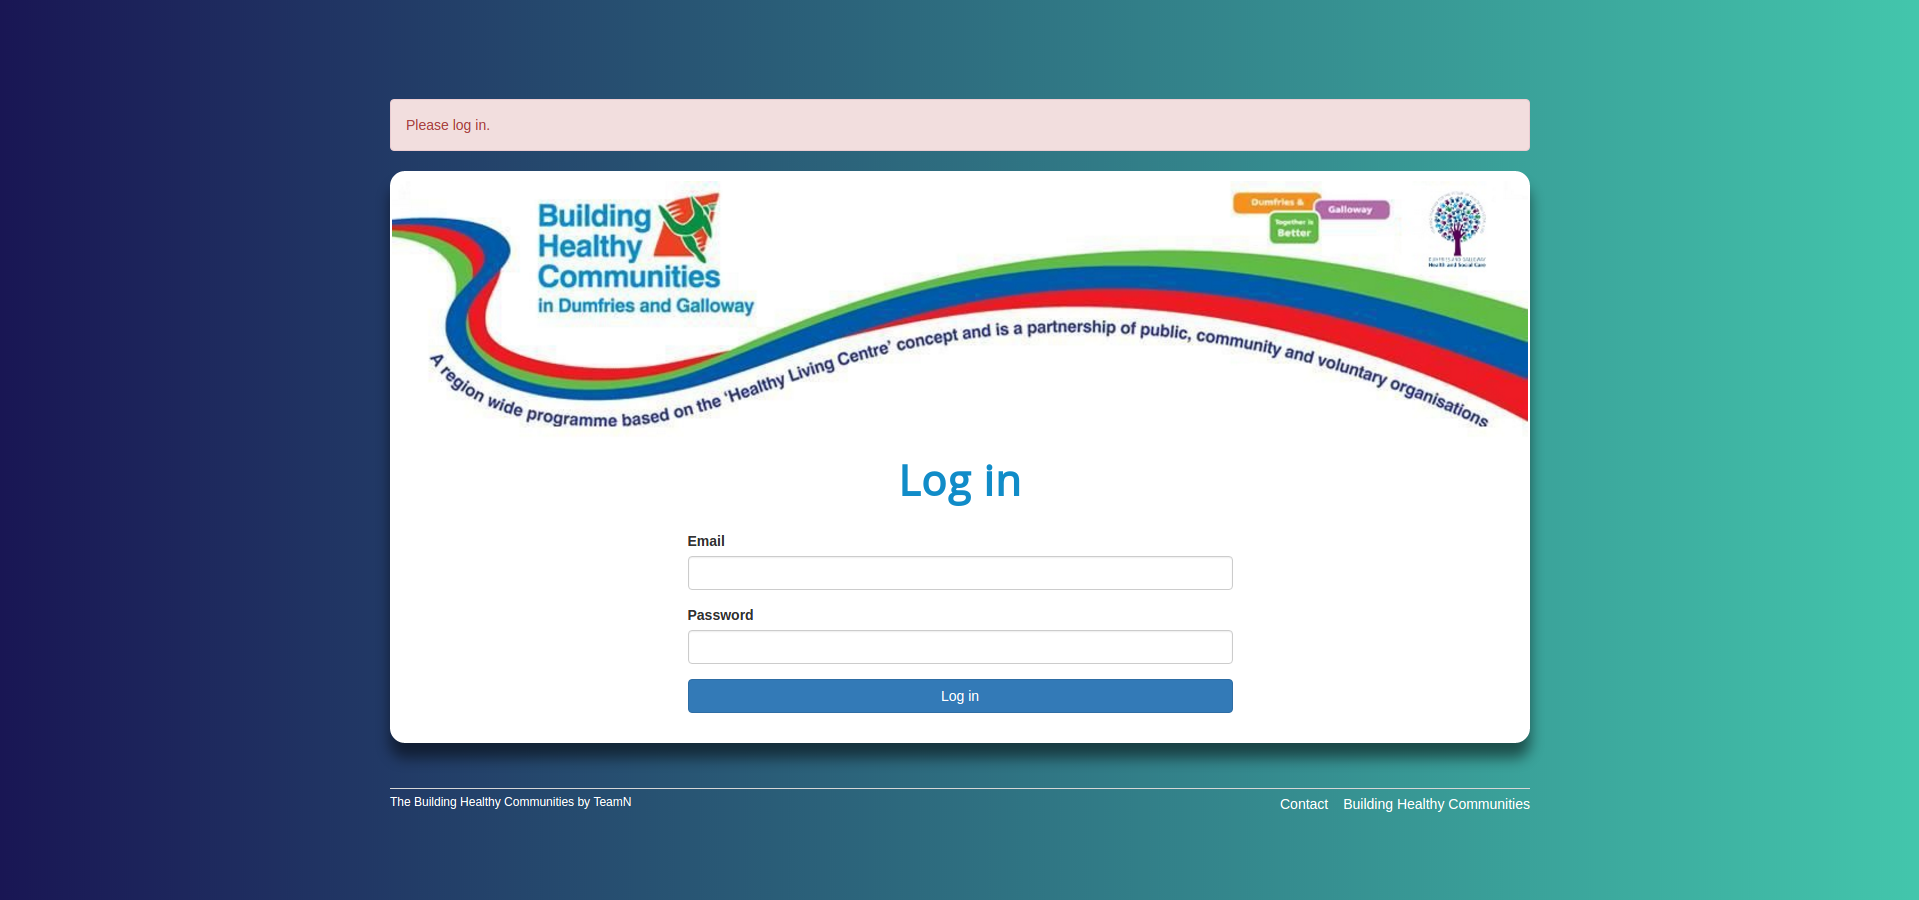
\includegraphics[width=\textwidth, height=\textheight, keepaspectratio]{loginscreen.png}}
 \caption{Login page}
 \label{fig:initialLogin}
\end{figure}

To login to the website, enter your email address and password. Until you do so, there is no way to access the website beyond this page. In the case that you have forgotten your email address and/or password, see \autoref{sec:contacts}: Contacts and Forgotten Passwords.

\pagebreak

\section{Home Page}
\label{sec:homepage}

Once logged in to the system, you will be presented with the home page, as seen in \autoref{fig:homePage}. From here, you can see an overview of all the initiatives you are enrolled in. You can see the information given for each initiative includes the name, description, location, and the names of the volunteers that run the initiative.

Above the initiatives there is a line with words to the effect of 'Your feedback is due in...' followed by a green 'Leave Feedback' button. This is the method of giving the 3 monthly feedback, as described in \autoref{sec:feedback}: Feedback.

Finally, at the top of the screen is the menu bar, seen in \autoref{fig:menuBar}. From here you can go between the home page and profile page (\autoref{sec:profile}), or log out.

\begin{figure}[h]
 \centerline{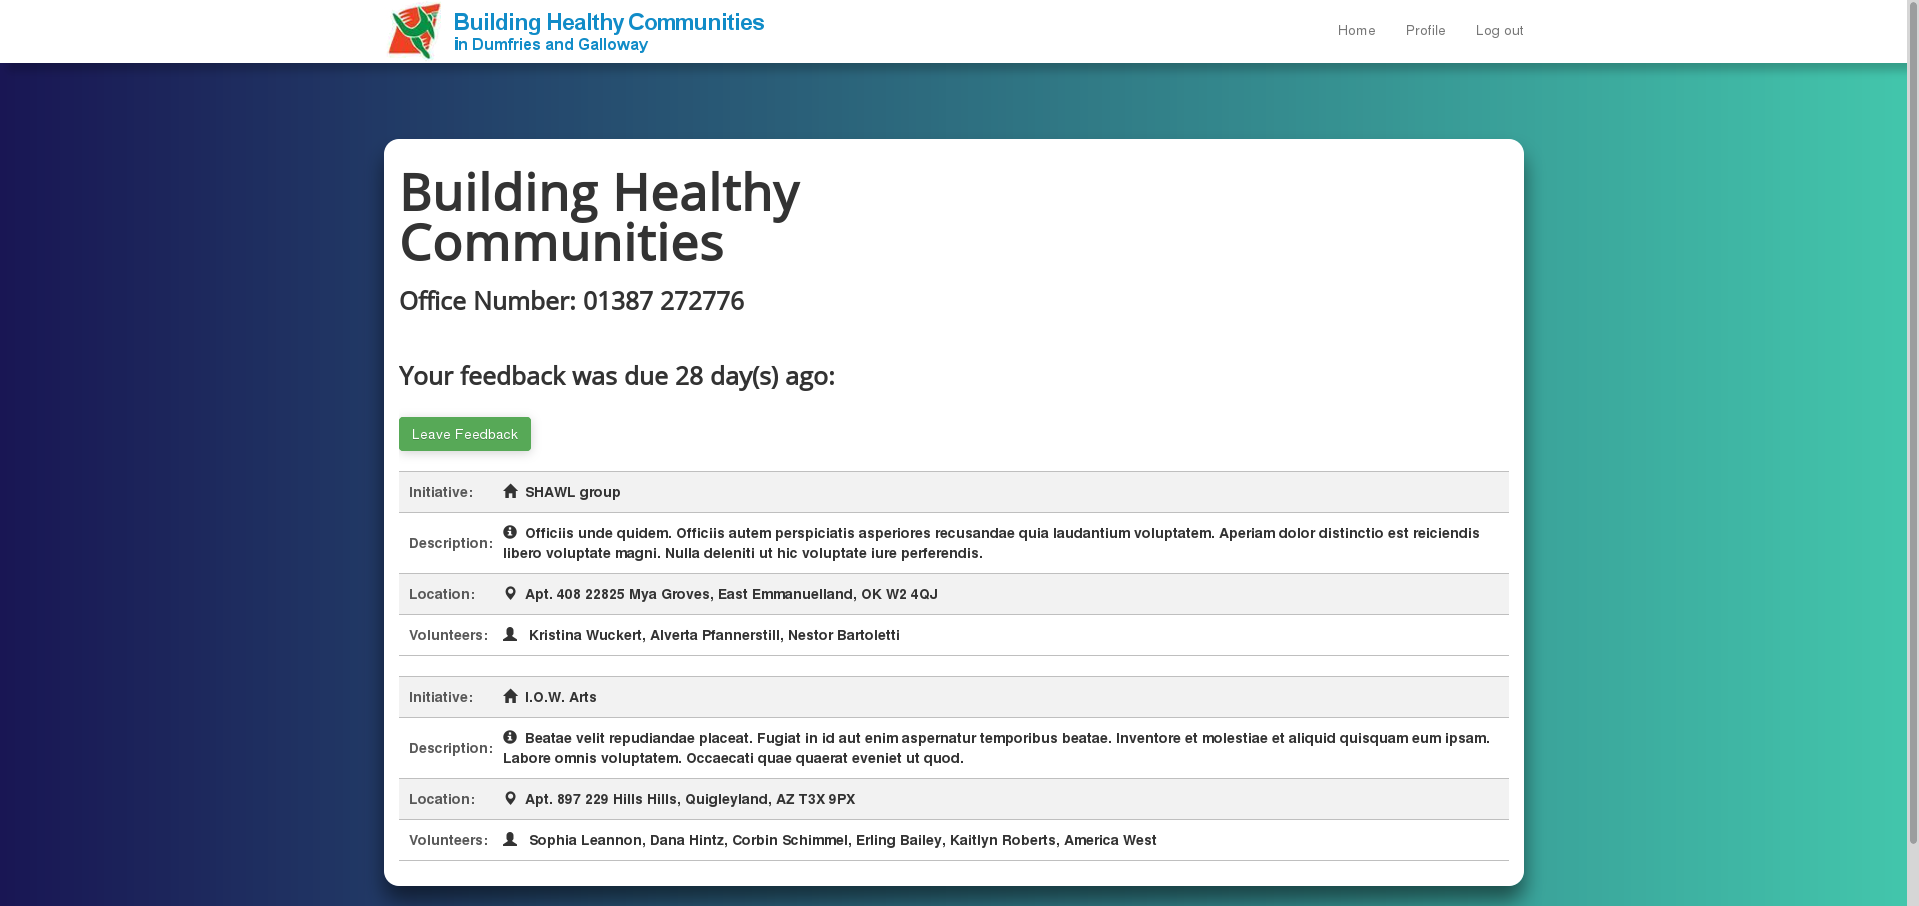
\includegraphics[width=\textwidth, height=\textheight, keepaspectratio]{homepage.png}}
 \caption{Home page}
 \label{fig:homePage}
\end{figure}

\begin{figure}[h]
 \centerline{
\includegraphics[width=\textwidth, height=\textheight, keepaspectratio]{menubar.png}}
 \caption{Menu bar}
 \label{fig:menuBar}
\end{figure}

\pagebreak

\section{Profile Page and Detail Changes}
\label{sec:profile}

The profile page, seen in \autoref{fig:profilePage} contains all the details the Building Healthy Communities system holds on you, from name and date of birth, to emergency contacts, to the direct funding you receive. As this data is protected, only you and system administrators can view it. However, you cannot modify this information yourself, though you may send a request for an admin to change it. 

To do this, click the blue 'Change Details' button near the top right of the page. This will take you to a small text box page (\autoref{fig:detailChange}) where you may type in the details that you want to be changed, and what you want them changing to. Double check that you have typed the details correctly, as the administrator needs to know they are accurate before making the change! It is possible that an administrator may contact you before making the change anyway, but better safe than sorry.

By scrolling down the details page, you can see a second section, seen in \autoref{fig:fundingInfo}. This lists all the indirect funding that the BHC programme receives related to your attendance. Indirect funding is received from various sources, either to fund a specific initiative (listed on the left), or to go towards initiatives geared towards those with particular conditions in the hope of improving their lives (listed on the right).

\begin{figure}[h]
 \centerline{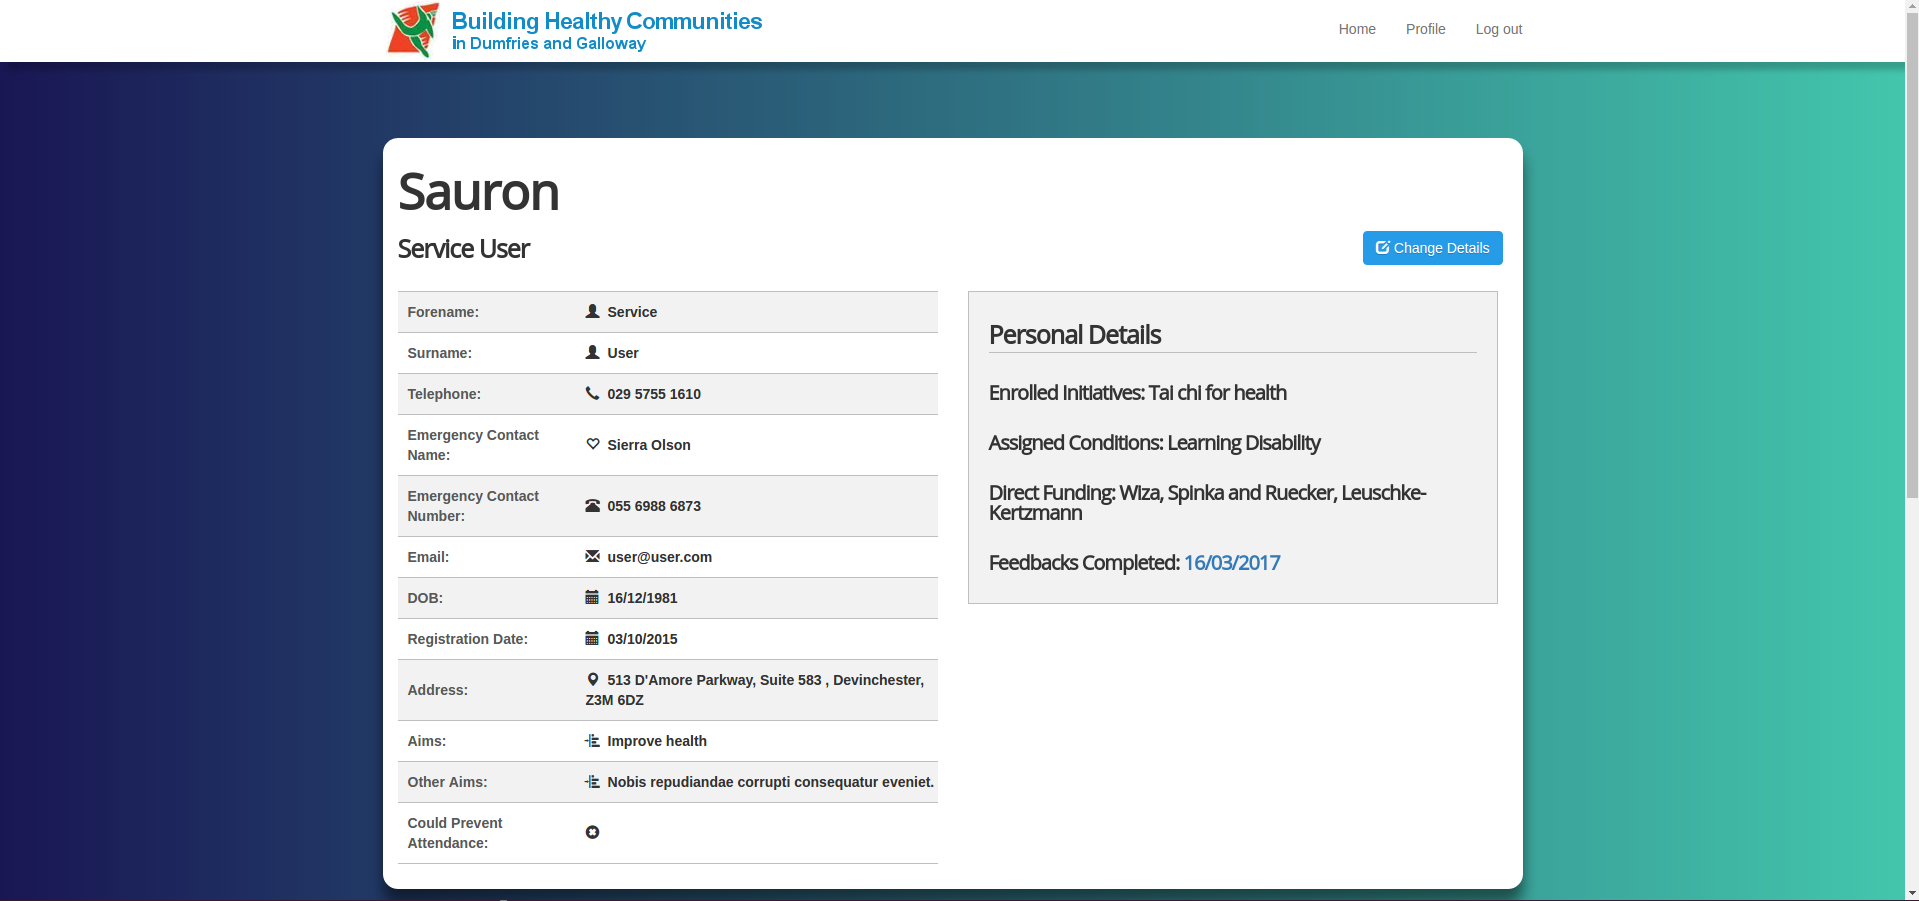
\includegraphics[width=\textwidth, height=\textheight, keepaspectratio]{profilepage.png}}
 \caption{Profile page}
 \label{fig:profilePage}
\end{figure}

\begin{figure}[h]
 \centerline{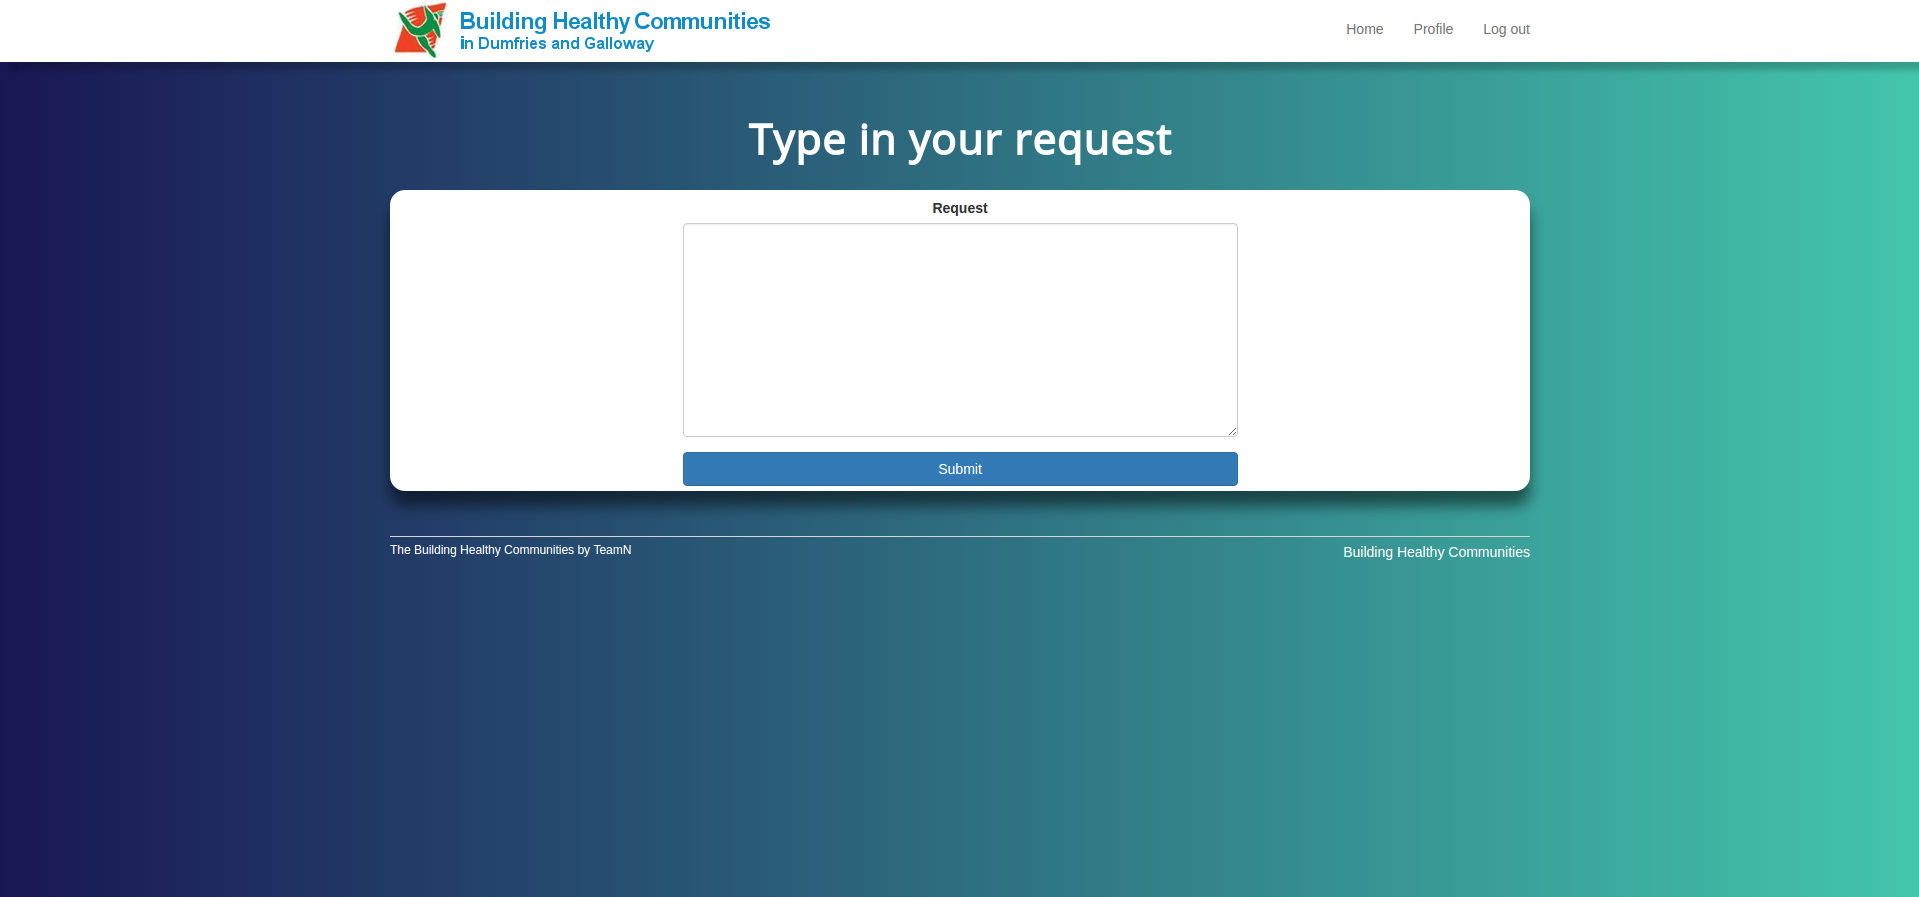
\includegraphics[width=\textwidth, height=\textheight, keepaspectratio]{detailchange.png}}
 \caption{Changing details request}
 \label{fig:detailChange}
\end{figure}

\begin{figure}[h]
 \centerline{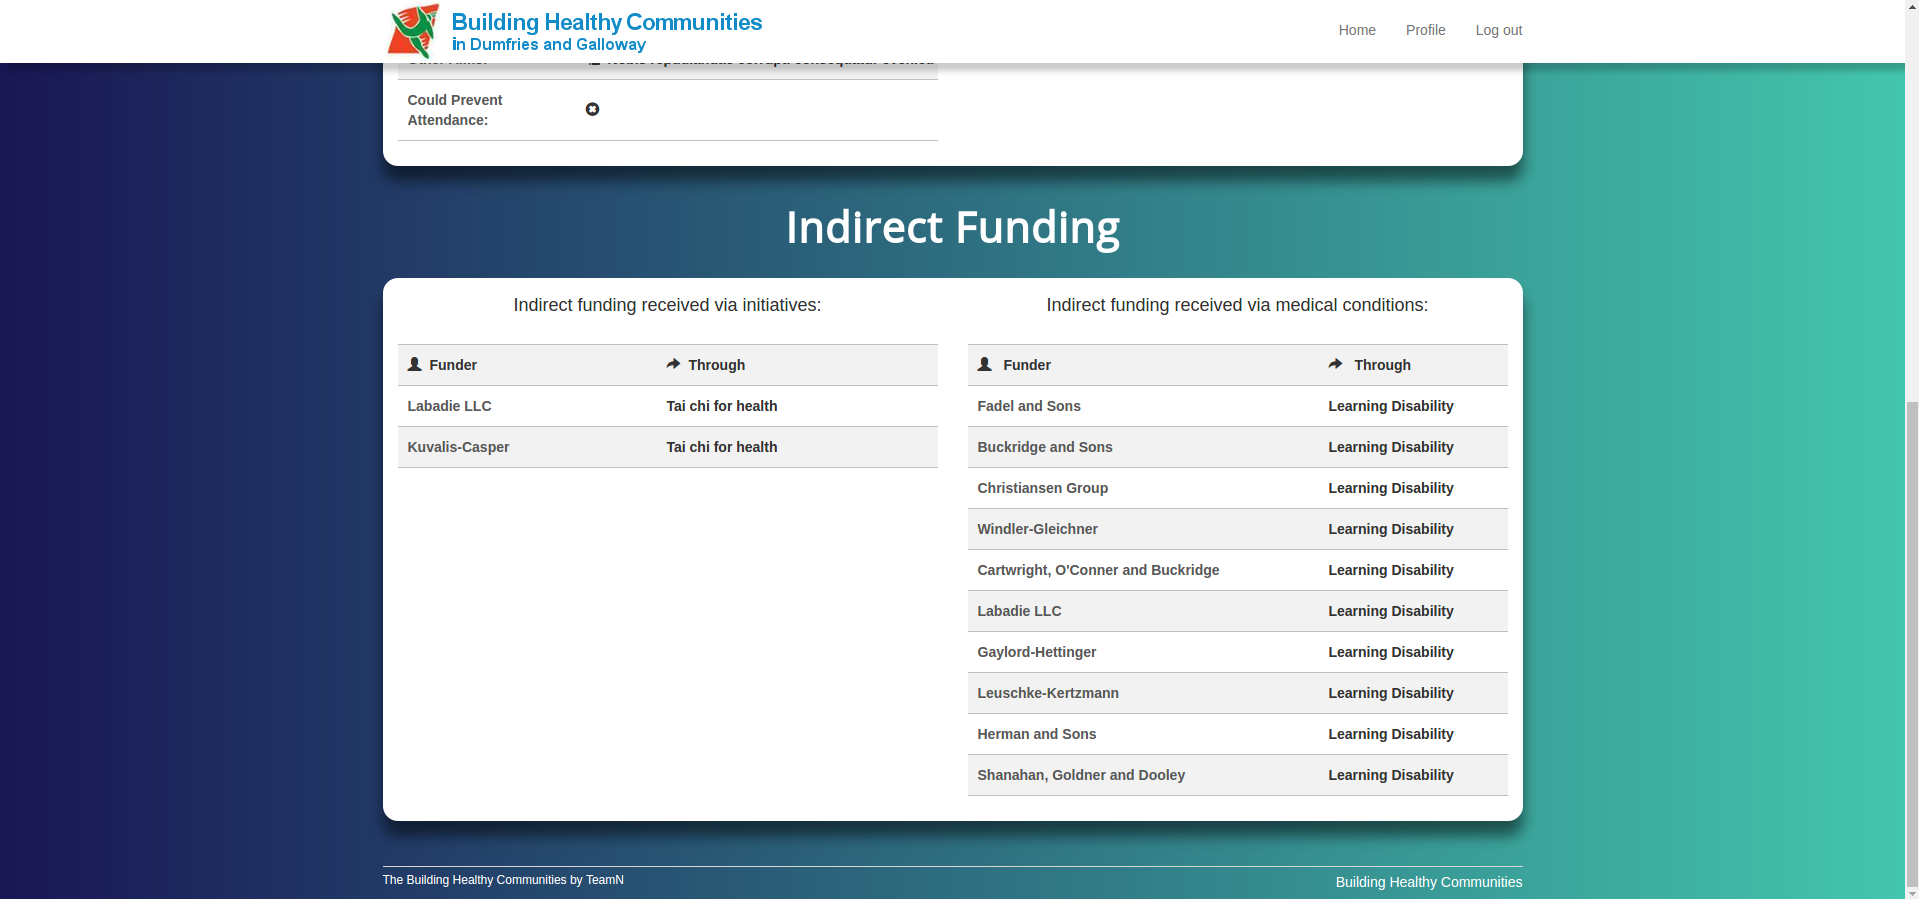
\includegraphics[width=\textwidth, height=\textheight, keepaspectratio]{fundinginfo.png}}
 \caption{Indirect funding info}
 \label{fig:fundingInfo}
\end{figure}

\section{Feedback}
\label{sec:feedback}

Leaving feedback is an important part of the BHC programme. It allows those running the programme to see the progress of everyone involved in the various initiatives. Feedback is usually left every three months, though this time can vary, and you may leave feedback at any time. To leave feedback, click the green 'Leave Feedback' button on the home page, and you will be taken to the feedback page, seen in \autoref{fig:feedbackPage}.

The feedback form asks you a standard set of questions about how you have been feeling, and how connected you feel to your community and local area. Your answers will be compared to your previous responses in an effort to guage how much the initiatives have affected you, either in a positive or negative way. You should answer the questions honestly, and do not be afraid to say you have gotten worse. The initiatives are there to help, and if they're doing something wrong, or there's something they can do, the people running them need to know!

\begin{figure}[h]
 \centerline{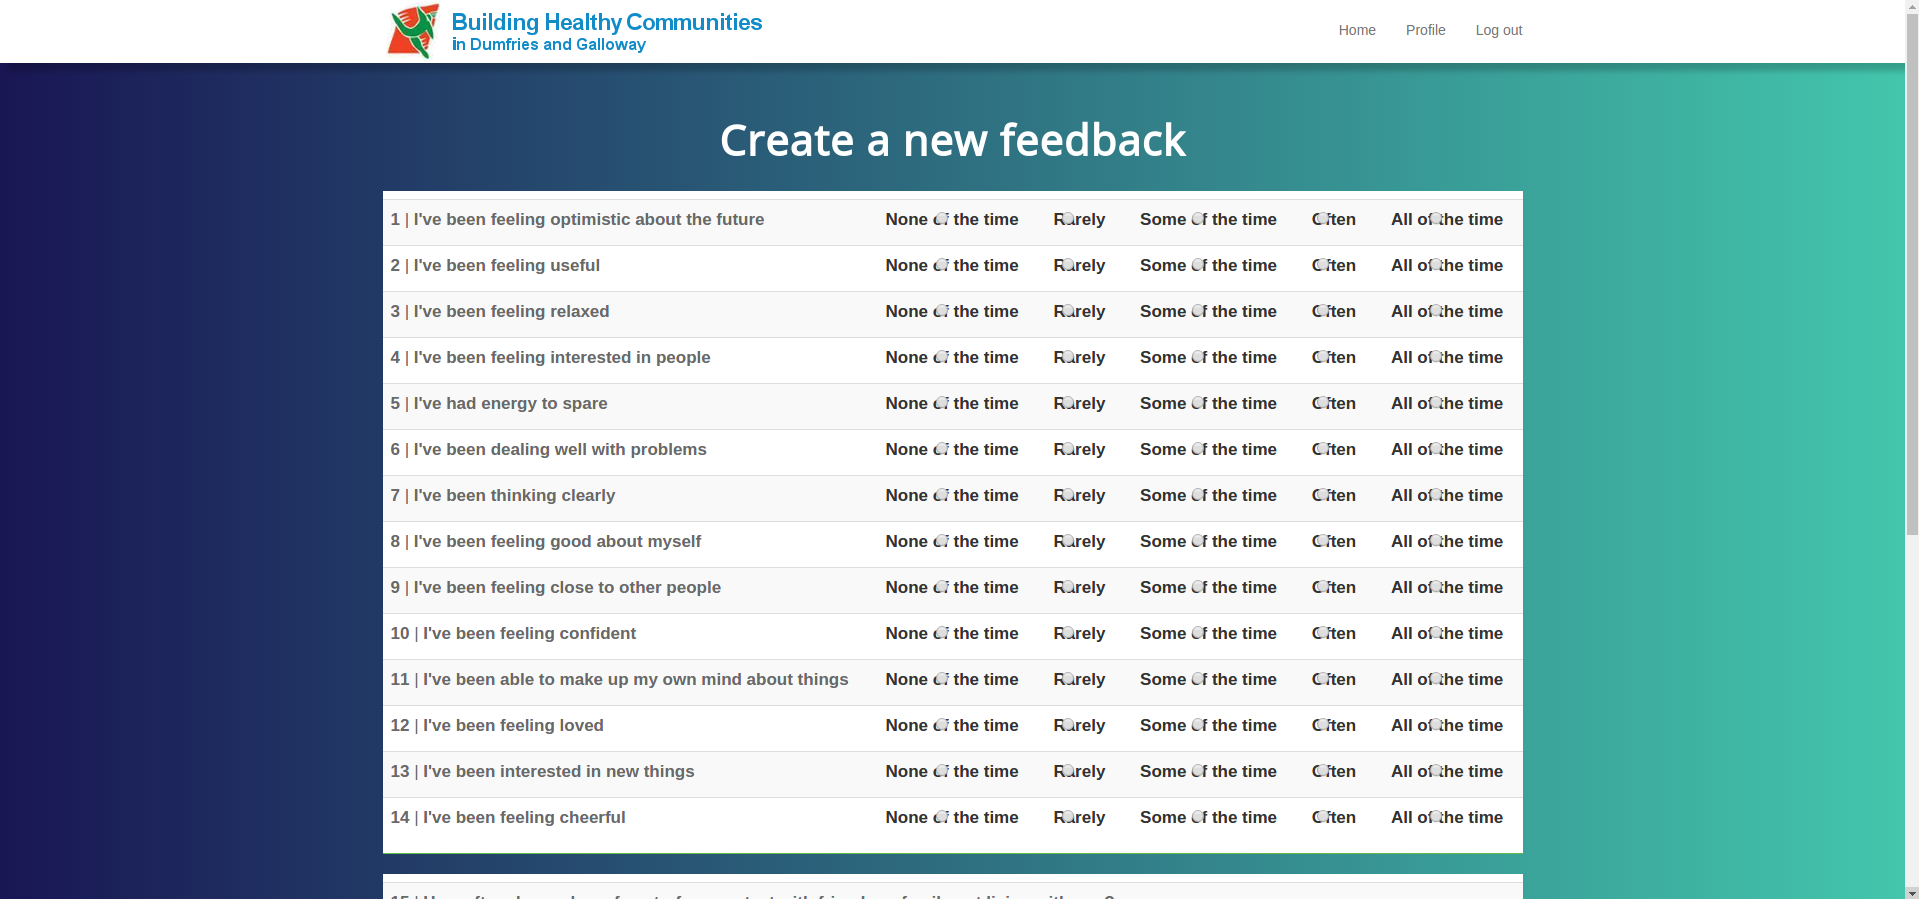
\includegraphics[width=\textwidth, height=\textheight, keepaspectratio]{feedbackpage.png}}
 \caption{Feedback page}
 \label{fig:feedbackPage}
\end{figure}

\pagebreak

\section{Contacts and Forgotten Passwords}
\label{sec:contacts}

If you want to find contact details for a given area, there is an easy way to do so. On the login page (you will have to log out if you are currently logged in), in the bottom right is the word 'Contact'. Clicking on this will bring up the contacts page, from which the addresses of the various area partnerships can be found, as seen in \autoref{fig:contactPage}. This page also includes the names and roles of people working there, and a telephone number. If you have forgotten your email address and/or password, you can call the number for your area and the team will try to help, asking you a few security questions (to make sure you're you!), before resetting your login details.

\begin{figure}[h]
 \centerline{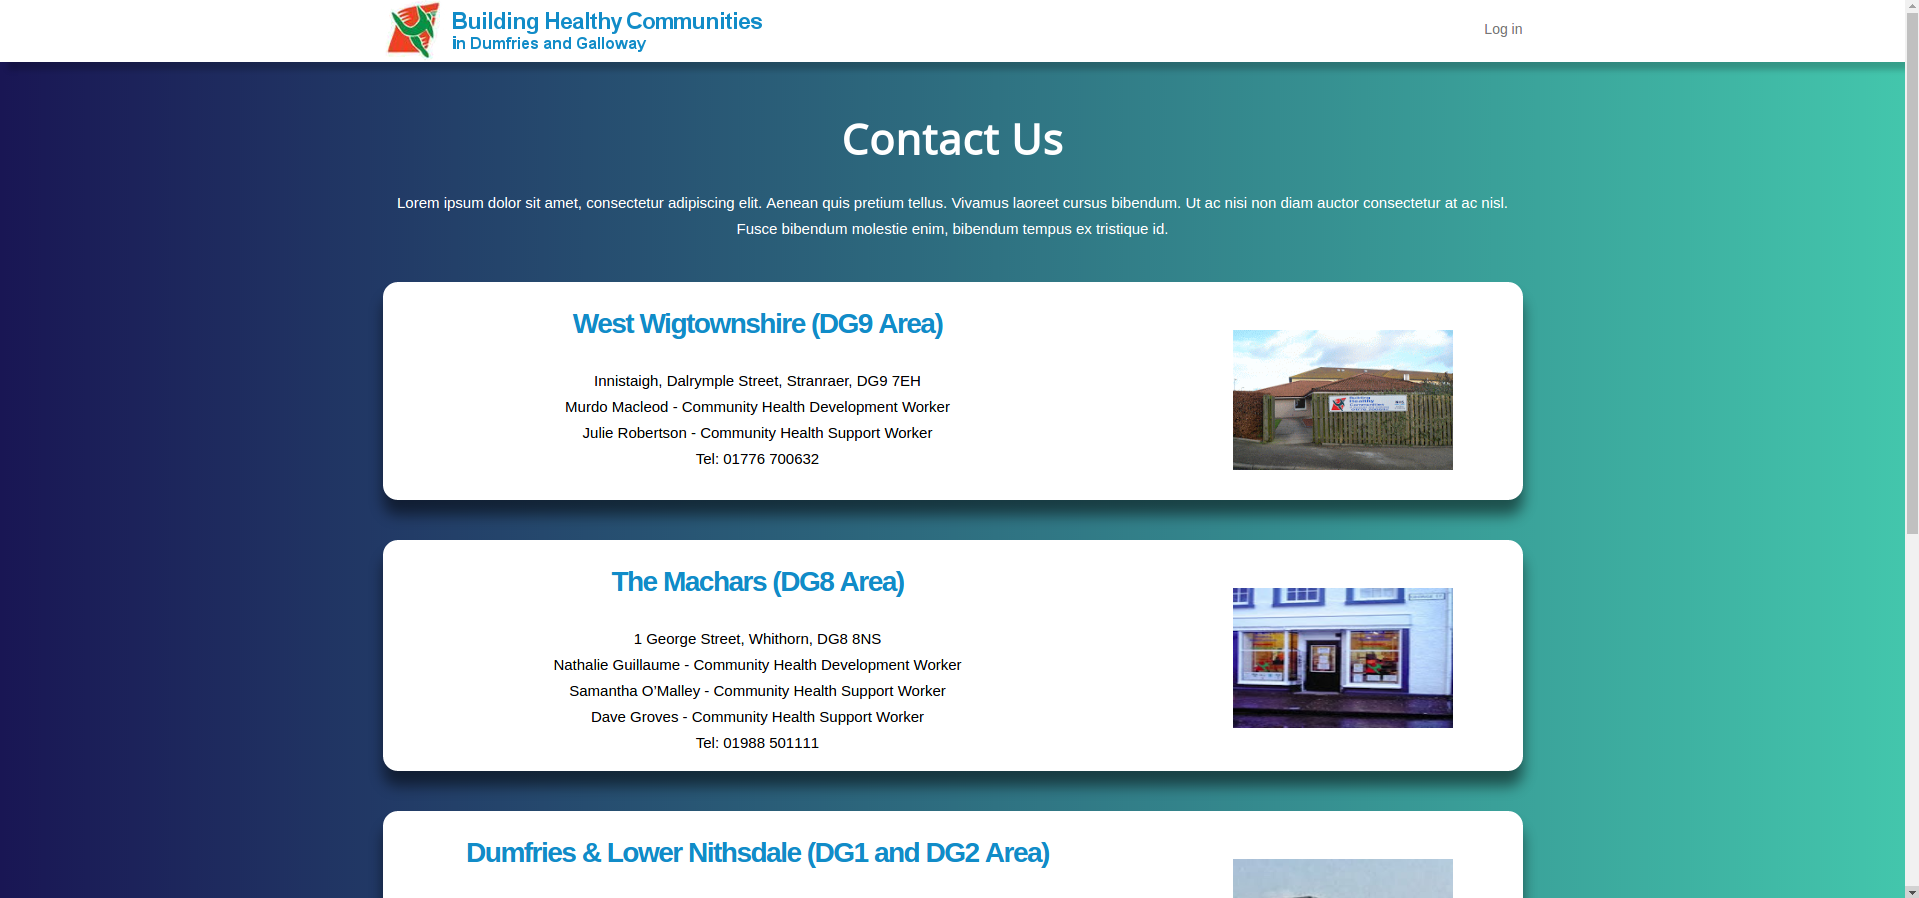
\includegraphics[width=\textwidth, height=\textheight, keepaspectratio]{contactpage.png}}
 \caption{Contact page}
 \label{fig:contactPage}
\end{figure}

\end{document}
